\chapter{Lecture}\label{part2:lec15} %%% 15
\markboth{\thechapter. Lecture}{\thechapter. Lecture}

We\pageoriginale were discussing the possibility of getting a root of
unity determined for the transformation of $\mathscr{V}_{11}'\left(\nu
\Big/ \dfrac{a \tau+ b}{c\tau +d}\right)$. There do exist methods for
determining this explicitly. Only we tried to carry out the analogue
with the special case as far as possible, not with complete
success. other methods exist. The first of these is due to Hermite,
done nearly 100 years ago. He used what are called Gaussian
sums. There are difficulties there too and we want to avoid
them. Another method is that of Dedekind using Dedekind sums.

In the special case of the transformation from $\tau$ to $\tau' =-
\frac{1}{\tau}$ we were faced with an elliptic substitution
$\left( \begin{smallmatrix} a & b\\ c &
  d\end{smallmatrix}\right)$. These are of two sorts:
\begin{enumerate}
\item $a+d=0$
\item $a+d=\pm 1$
\end{enumerate}
 In both cases we can completely forget about the root of unity if we
 remember the following fact. Our formula had the following shape:
\begin{equation*}
  \mathscr{V}_{11}' \left(0 \Big/ \frac{a \tau+b}{c\tau+d} \right)=
  \sqrt{\frac{c\tau+d}{i}} \cdot \frac{c \tau+d}{i} \rho (a, b, c, d)
  \mathscr{V}_{11}' (0 /\tau) \tag{*}\label{part2:lec15:eq*} 
\end{equation*}
where $\rho$ is a root of unity which is completely free of $\tau$. we
can then get things straightened out. We have only to consider the
fixed points of the transformation given by
$$
\xi= \frac{a-d \pm \sqrt{(a+d)^2-4}}{2c}
$$

Put\pageoriginale $\xi$ on both sides of the formula; since $\xi =
\dfrac{a \xi +b}{c \xi +d}$, both sides look alike and
$\mathscr{V}_{11}'$ does not vanish for appropriate $\tau$ in the
upper half-plane (we may take $c> 0$), so that $\rho$ is given directly
by the formula.

\begin{case}\label{part2:lec15:case1}
  $a+d=0$
  $$
  \xi = \frac{- 2d \pm \sqrt{-d}}{2c} =  \frac{- d + i}{c}
  $$
  (reject the negative sign since we want a point in the upper
  half-plane). 
  \begin{align*}
    \frac{c \xi+d}{i} &= \frac{i}{1} = i\\
    \therefore \qquad \mathscr{V}_{11}' (0 / \xi) & = \rho (a, b, c,
    d) \mathscr{V}_{11}' (0/\xi)\qquad 
  \end{align*}
  So $\rho (a, b, c, d)=1$ and remains 1 in the general formula when
  we go away from $\xi$.
\end{case}

\begin{case}\label{part2:lec15:case2}
  $a+d=\pm 1$
  \begin{align*}
    \xi & = \frac{\pm 1 - 2d+ \sqrt{-3}}{2c}\\
    \therefore \qquad c \xi + d & = \frac{\pm 1+ i \sqrt{3}}{2}=
    e^{\pi i /3} ~\text{or}~ e^{2 \pi i /3}\\
    \frac{c \xi+d}{i} & = e^{\pi i /3- \pi i /2} ~\text{or}~ e^{2 \pi
      i /3 - \pi i /2}\\
    & = e^{\pm \pi i /6}\\
    \sqrt{\frac{c \xi +d}{i}} & = e^{\mp \pi i /12}
  \end{align*}
\end{case}

Putting\pageoriginale $\xi$ on both sides of (\ref{part2:lec15:eq*}), 
$$
1= e^{\mp \pi i /4} \rho (a, b, c, d)
$$
$\therefore$ \hspace{2cm} $\rho (a, b,c, d)= e^{\pm \pi i /4}$

when $a+d= \pm 1$, (we may take $c>0$; the case $c=0$ is uninteresting
and if $c<0$ we can make it $c>0$).

There are unfortunately no more cases like these.

\noindent \textbf{Parabolic case.} The analysis here is a little
longer but it is worth while working it out. Now $a+d= \pm 2$, and
there is only one fixed point
$$
\xi= \frac{a-d}{2c} - \frac{- 2d\pm 2}{2c} = \frac{- d \pm 1}{c} = -
\frac \delta \gamma
$$
where $(\gamma, \delta)=1$ and we may choose $\gamma>0$. The fixed
point is now a rational point on the real axis. We try to approach
it. This is a little difficult because we do not know what the
function will do thee. But by an auxiliary transformation we can throw
this point into the point at infinity. Consider the auxiliary
transformation
$$
T= \frac{A \tau + B}{\gamma \tau + \delta}, 
\begin{vmatrix} A & B\\ \gamma &\delta \end{vmatrix}=1
$$

The denominator becomes zero for $\tau = \xi$. Let
$$
T'= \frac{A \tau' + B}{\gamma \tau' + \delta}
$$
(notice\pageoriginale that $\gamma$ and $\delta$ have got something
to do with the properties of two other numbers $c$, $d$). Now (*)
gives
\begin{align*}
  \mathscr{V}_{11}'(0/T) & = \left(\sqrt{\frac{\gamma \tau + \delta}{i}}
  \right)^3 \rho (A, B, \gamma, \delta) \mathscr{V}_{11}' (0/ \tau),\\
  \mathscr{V}_{11}' (0/T') & = \left(\sqrt{\frac{\gamma \tau' + \delta}{i}}
  \right)^3 \rho (A, B, \gamma, \delta) \mathscr{V}_{11}' (0/ \tau').  
\end{align*}

Dividing, we get
\begin{equation*}
  \frac{\mathscr{V}_{11}' (0/ T')}{\mathscr{V}_{11}'(0/ T)} =
  \left( \frac{\sqrt{\frac{\gamma \tau'+\delta}{i}}}{\sqrt{\frac{\gamma \tau
        + \delta}{i}}}\right)^3 \frac{\mathscr{V}_{11}' (0/
    \tau')}{\mathscr{V}_{11}' (0/ \tau)} \tag{1}\label{part2:lec15:eq1}
\end{equation*}

The left side gives the behaviour at infinity. We cannot of course put
$\tau = \xi$. Put $\tau = \xi + it$, $t > 0$, and later make $t \to
0$. $\tau$ is a point in the upper half-plane.
\begin{align*}
  \tau - \xi & = it,\\
  \tau' - \xi & = \frac{a \tau+b}{c\tau +d} - \frac{a \xi +b}{c \xi
    +d}\\
  & = \frac{ \tau - \xi}{(c \tau +d)(c \xi +d)}\\
  & = \frac{i t}{1 \pm i ct}
\end{align*}

This is also in the upper half-plane. $\tau' \to \xi$ as $t \to 0$

Let us calculate $T$ and $T'$. For this consider

\begin{align*}
  T' - T & = \frac{A \tau'+B}{\gamma \tau' + \delta} - \frac{A \tau +
    B}{\gamma \tau + \delta}\\
  & = \frac{\tau' - \tau}{(\gamma \tau' + \delta)(\gamma \tau +
    \delta)}\\
  & = \mp \frac{c}{\gamma^2}
\end{align*}\pageoriginale

This is quite nice; the difference is a real number.
\begin{align*}
  T & = \frac{A \tau + B}{\gamma \tau + \delta} = \frac{A (\xi + i t)+
    B}{\gamma (\xi + i t)+ \delta}\\
  & = \frac{A i t+ A \xi + B}{\gamma i t}, ~\text{since}~ \gamma \xi +
  \delta =0,\\
  & = \frac{A}{\gamma} + \frac{ -A \frac{\delta}{\gamma}+ B}{\gamma i
    t}\\
  & = \frac A \gamma + \frac{B \gamma - A \delta}{\gamma \tau t}\\
  & = \frac A \gamma + \frac{1}{\gamma^2 t}, ~\text{since}~ B \gamma -
  A \delta =- 1
\end{align*}
$\to i \infty$ (along the ordinate  $x = \frac{A}{\gamma}$) as $t \to
0$
\begin{align*}
  T' = & \frac{A}{\gamma} \pm \frac{c}{\gamma^2} + \frac{i}{r^2 t}\\
  & \to i \infty ~\text{as}~ t \to 0
\end{align*}

Now\pageoriginale recall the infinite product formula
$$
\mathscr{V}_{11}' (0/ T)= 2 \pi i e^{\pi i T/4} \prod^\infty_{n=1} (1-
e^{2 \pi i n T})^3
$$

Let \qquad $T= \frac{A}{\gamma} + \frac{i}{\gamma^2 t}$. Then 
\begin{align*}
  e^{2 \pi i n T} & = e^{2 \pi i n A/\gamma} e^{- 2 \pi n t /\gamma^2}
  \to 0\\
  \therefore \qquad \mathscr{V}_{11}' (0/T) & = 2 \pi i e^{\pi i T/4}
  (\text{a factor tending to 1})
\end{align*}

We do not know what happens to $e^{\pi i T/4}$. But we need only the
quotient. So
\begin{align*}
  \frac{\mathscr{V}_{11}' (0/\tau)}{\mathscr{V}_{11}' (0/ \tau)} & \sim
    e^{\pi i (T' - T)/4}\\
    & = e^{\mp \pi i c/4 \gamma^2} \tag{2}\label{part2:lec15:eq2}
\end{align*}

Consider similarly the quotient $\mathscr{V}_{11}'
(0/\tau')/\mathscr{V}_{11}' (0/\tau)$. We have, since $\gamma \xi +
\delta =0$, 
$$
\frac{\gamma \tau +\delta}{i} = \frac{\gamma(\xi + i t)+ \delta}{i} =
  \gamma^t 
$$
or $\sqrt{\dfrac{\gamma \tau + \delta}{i}} = \sqrt{\nu t}$, where we take
the positive square root
\begin{align*}
\frac{\gamma \tau' + \delta}{i} & = \frac{\gamma \left(\xi + \frac{it}{1 \pm i
    c t}\right)+ \delta}{i} = \frac{\gamma t}{1 \pm i ct}\\
\therefore \quad \sqrt{\frac{\gamma \tau' + \delta}{i}} & = \sqrt{r t}
\sqrt{\frac{1}{1\pm i ct}} \quad \text{(both branches principal)}\\
& \quad \sim \sqrt{\gamma t} ~\text{as}~ t \to 0.
\end{align*}

Hence\pageoriginale the quotient $\sqrt{\dfrac{\gamma \tau'+ \delta}{i}}\Big/
\sqrt{\frac{\gamma \tau + \delta}{i}}$ behaves like 1.

And so we have what we were after:
\begin{align*}
  \frac{\mathscr{V}_{11}'(0/ \tau')}{\mathscr{V}_{11}' (0/ \tau)} &
  \to e^{\mp \pi i c /4 \gamma^2} ~\text{as}~ t \to 0 \tag{3}\label{part2:lec15:eq3}\\
  \frac{c \tau +d}{i} & = \frac{c (\xi + i t)+d}{i} =
  \frac{\frac{a-d}{2}+ c it +d}{i}\\
  & = \frac{a + \frac{d}{2} + c it}{i} = \pm \frac{1+ c i t}{i}\\
  & = \mp i + c t\\
  & \to \mp i ~\text{as}~ t \to 0.
\end{align*}

What will the square root of this do?

\medskip
\noindent 
\begin{minipage}[c]{4.5cm}
  $\sqrt{\dfrac{c \tau+d}{i}} = \sqrt{ct\mp i}$, and this does lie in
  the proper half plane because $ct > 0$. For small $t$ it will be very
  near the imaginary axis near $\mp i$. So the square root lies in the
  sector, in the lower half plane if we choose $\sqrt{-i} = e^{- \pi
    i/4}$, and in the upper half-plane if we choose $\sqrt{+i}= e^{\pi i/4
  }$ Hence $\sqrt{\dfrac{c \tau +d}{i}}\to e^{\mp \pi i/4}$ as $t \to
  0$. 
\end{minipage}
\begin{minipage}[c]{5.5cm}
  \begin{figure}[H]
    \centering{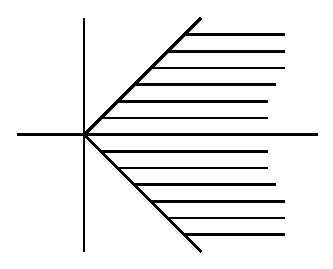
\includegraphics{vol2-figures/fig2.20.eps}}
  \end{figure}
\end{minipage}

Using\pageoriginale this fact as well as (\ref{part2:lec15:eq2}) and
(\ref{part2:lec15:eq3}) in (\ref{part2:lec15:eq*}) we get 
\begin{align*}
  e^{\mp \pi i c/4\gamma^2} & = e^{\mp 3 \pi i /4} \rho (a, b, c, d)\\
  \therefore \qquad\qquad  \rho (a, b, c, d) & = e^{\mp} \frac{\pi i}{4}
  (c/\gamma^2-3)\hspace{2cm} 
\end{align*}

We observe that the common denominator $(\gamma, \delta)=1$ plays a
role, however $a$ and $b$ do not enter.

\medskip
\noindent \textbf{Hyperbolic case.} The thing could also be partly
considered in the hyperbolic case. It will take us into deeper things
like real quadratic fields and we do not propose to do it.

Let us return to what we had achieved in the specific case. We had a
formula for $\eta (\tau)$:
$$
\eta(\tau') = \sqrt{\frac{c \tau+d}{i}} \epsilon(a, b, c, d) \eta (\tau),
$$
where $\epsilon (a, b, c, d)$ is a 24th root of unity. This shape we have
in all circumstances. The difficulty is only to compute $\epsilon$. We
shall not determine it in general, and we can do away with it even for
the purpose of partitions by using a method developed recently by
Selberg. 

However in each specific case we can compute $\epsilon$.
$$
\eta \left( - \frac{1}{\tau}\right)= \sqrt{\frac{\tau}{i}} \eta (\tau)  
$$

Now  
\begin{align*}
  \eta (\tau) & = e^{\pi i \tau/12} \prod^{\infty}_{n=1} (1- e^{2 \pi
    i n \tau}),\\
  \eta (\tau + b) & = e^{\pi i b/12} \eta(\tau)
\end{align*}

Out\pageoriginale of these two facts we can get every other one,
because the two substitutions
$$
S= \begin{pmatrix} 1 & 1\\  0 & 1 \end{pmatrix}, \qquad 
T= \begin{pmatrix} 0 & -1\\ 1 & 0 \end{pmatrix}
$$
form generators of the full modular group. This can be shown as
follows. Take $c> 0$.
\begin{align*}
  a \tau + b & = q_0 (c \tau +d)- a, \tau - b_1, c > |a_1|,\\
  \text{or} \hspace{2cm} \frac{a \tau +d}{c \tau +d} & = q_0 -
  \frac{a_1 \tau + b_1}{c \tau +d}, \quad 
  \begin{vmatrix} c & d\\ a_1 & b_1 \end{vmatrix} =1
\end{align*}
(if $a<0$ this step is unnecessary). Similarly
$$
\frac{c \tau +d}{a_1 \tau + b_1}= q_1 - \frac{a_2 \tau + b_2}{a_1 \tau
  + b_1} 
$$

We thus get a continued fraction expansion. The partial quotients get
similar and simpler every time and end with $\dfrac{\tau +b}{0 +1} =
\tau + q_k$. so we can go back and take linear combinations; all that
we have to do is either to add an integer to $\tau$ or take $-
1/\tau$. 

As an example, let us consider
$$
\eta \left(\frac{3 \tau+4}{2 \tau+3} \right)
$$

Let us break $\dfrac{3 \tau +4}{2 \tau +3}$ into simpler
substitutions, 
\begin{align*}
  \tau_3 & = \frac{3 \tau+4}{2 \tau+3} =1 - \frac{1}{\tau_2},\\
  \tau_2 & = -2 + \tau_1;\\
  \tau_1 & = - \frac{1}{\tau +1}\\
  \eta(\tau_1) & = \eta \left( - \frac{1}{\tau+1}\right) =
  \sqrt{\frac{\tau +1}{i}} \eta (\tau+1)\\
  & = \sqrt{\frac{\tau+1}{i}} e^{\pi i /12} \eta (\tau).\\
  \eta (\tau_2) & = \eta (\tau_1 -2) = e^{- \pi i /6} \eta(\tau_1)\\
  & = \sqrt{\frac{\tau+1}{i}} \cdot e^{- \pi i /12} \eta(\tau)\\
  \eta \left(- \frac{1}{\tau_2} \right) & = \sqrt{\frac{\tau_2}{i}}
  \eta (\tau_2)\\
  & = \sqrt{\frac{\tau+1}{i}} \sqrt{\frac{\tau_2}{i}} e^{- \pi i /12}
  \eta (\tau)
\end{align*}

The\pageoriginale two square roots taken separately are each a principal branch, but
taken together they may exceed one. We can write this as
\begin{align*}
  \eta\left(- \frac{1}{\tau_2} \right) & = \sqrt{\frac{\tau+1}{i}}
  \sqrt{\frac{-2 - \frac{1}{\tau+1}}{i}} e^{- \pi i /12} \eta (\tau)\\
    & = \sqrt{\frac{\tau+1}{i}} \sqrt{\frac{- 2 \tau -3}{i (\tau +1)}}
    e^{- \pi i /12} \eta(\tau)\\
    & = \sqrt{\frac{- 2 \tau-3}{-1}} e^{- \pi i /12} \eta (\tau)\\
    & = \pm \sqrt{3+ 2 \tau} e^{- \pi i /12} \eta (\tau)
\end{align*}

Here\pageoriginale we are faced with a question: which square root
are we to take? 

We write $\sqrt{3+ 2 \tau}= e^{\pi i /4} \sqrt{\frac{2 \tau +3}{i}}$

Let us look into each root singly. For $\tau = it$ where do they go?
\begin{align*}
  \sqrt{\frac{\tau+1}{i}} & = \sqrt{\frac{i t+1}{i}}\\
  & \quad  \to \infty ~\text{with argument}~ 0 ~\text{as}~ t \to \infty.\\
  \sqrt{\frac{- 2 \tau -3}{i (\tau +1)}} & = \sqrt{\frac{-2 i t -3}{i
      (\tau +1)}} \to \sqrt{2 i} ~\text{as}~ t \to \infty,\hspace{1cm}\\
  \text{or its argument} \hspace{2cm}& = \pi/4
\end{align*}

The product $\sqrt{\dfrac{\tau+1}{i}} \sqrt{\dfrac{- 2\tau -3}{i (\tau
    +1)}}$ has here argument $\pi/4$, so that it continues to be the
principal branch. Of course in a less favourable case, if we had two
other arguments, together they would have run into something which was
no longer a principal branch. Finally,
$$
\eta \left(\frac{3 \tau+4}{2 \tau+3} \right)= e^{\pi i /4}
\sqrt{\frac{2 \tau+3}{i}} \eta (\tau)
$$
and here there is no ambiguity. Actually in every specific case that
occurs one can compute step and make sure what happens. 

There does exist a complete formula which determines $\epsilon (a, b, c, d)$
explicitly by means of Dedekind sums $S(h, k)$. 

